% Cara menghitung V1 dari V dan c (contoh angka 4 dimensi), beserta gambar geometrinya.
% Kompilasi (dari folder ini): pdflatex cosine_hitung.tex && pdftoppm -png -r 300 -singlefile cosine_hitung.pdf cosine_hitung
\documentclass[border=6pt]{standalone}
\usepackage{amsmath}
\usepackage{amssymb}
\usepackage{mathptmx}
\usepackage{tikz}
\usetikzlibrary{arrows.meta, calc, positioning}

\definecolor{ink}{HTML}{3A3936}
\definecolor{muted}{HTML}{8A8984}
\definecolor{modelE}{HTML}{2A78D6}\definecolor{modelF}{HTML}{DCE9F9}
\definecolor{augE}{HTML}{EB6834}

\tikzset{
  every node/.style={font=\normalsize, text=ink, align=left},
  title/.style={font=\large\bfseries, anchor=west},
  box/.style={rectangle, rounded corners=3pt, line width=0.8pt, draw=muted, fill=white, inner sep=6pt, text width=118mm, anchor=north west},
  vec/.style={-{Stealth[length=3mm]}, line width=1.8pt},
  flow/.style={-{Stealth[length=2.3mm]}, line width=0.8pt, draw=ink},
}

\begin{document}
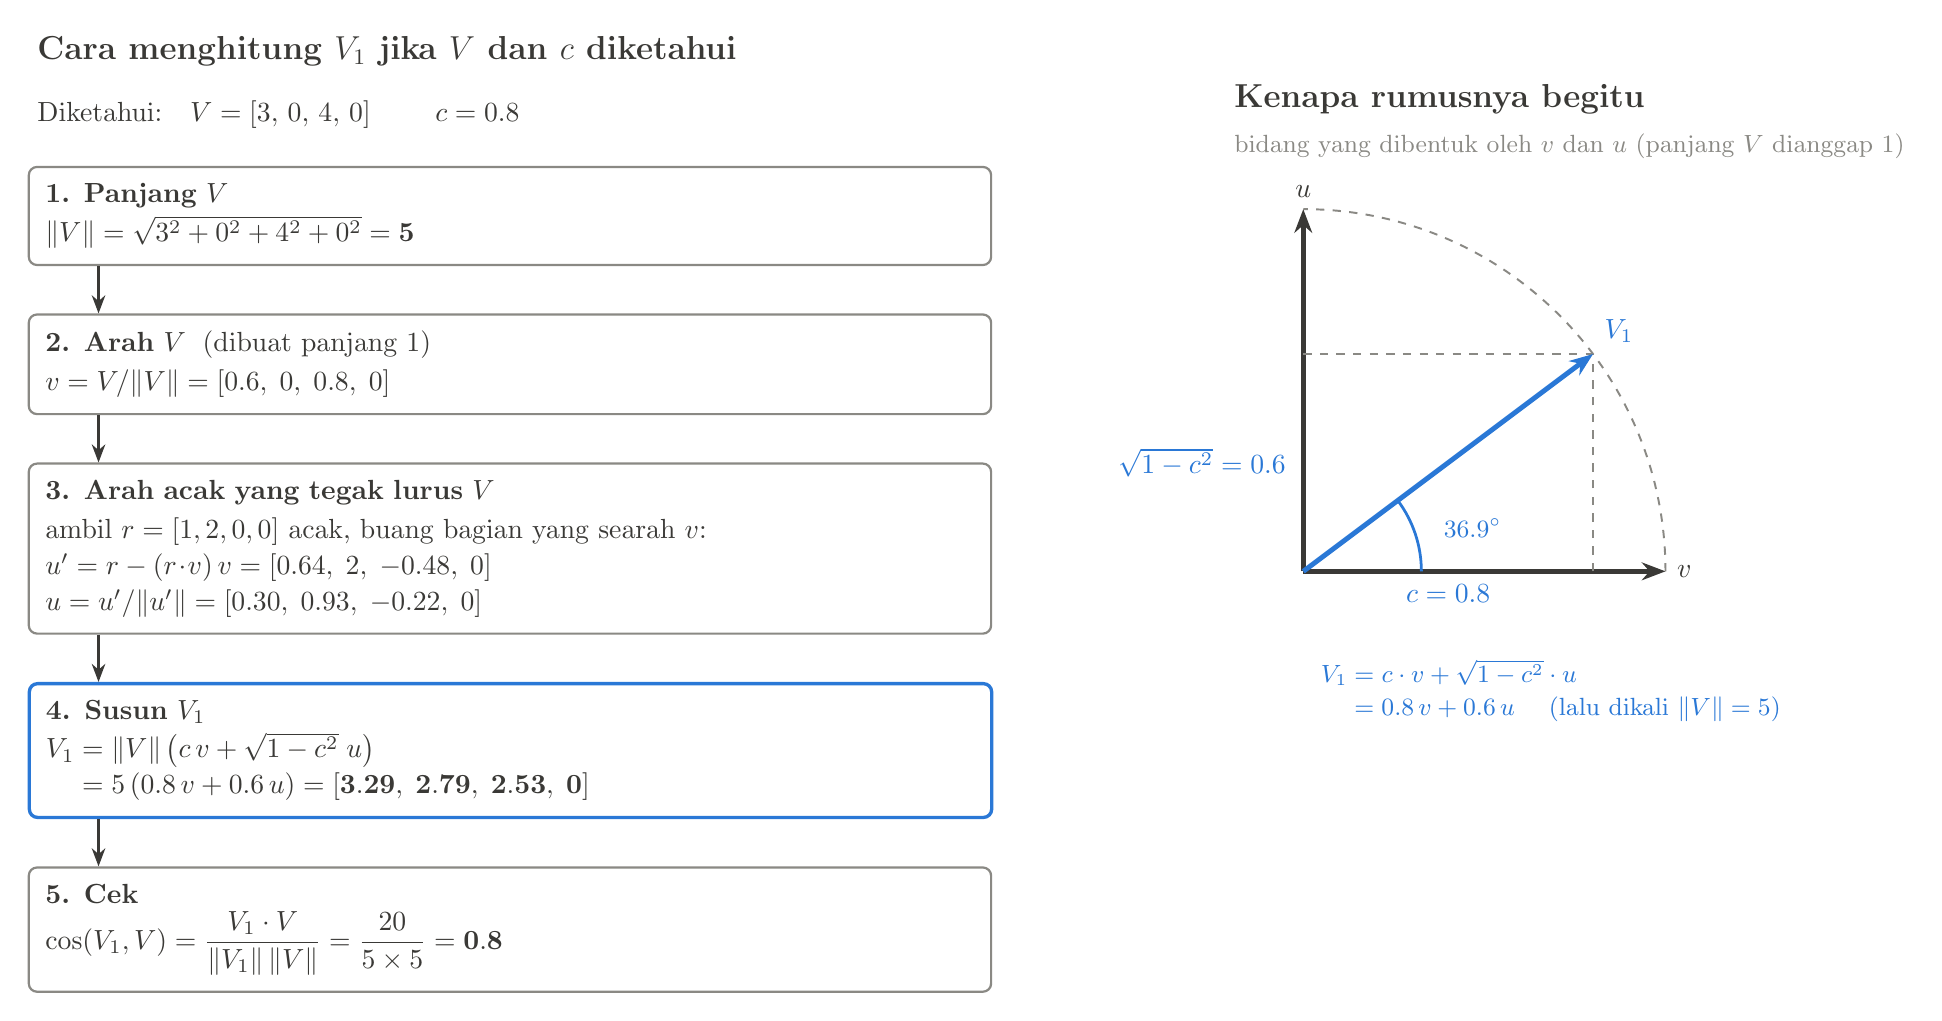
\begin{tikzpicture}

\node[title] at (0,0.6) {Cara menghitung $V_1$ jika $V$ dan $c$ diketahui};
\node[anchor=west] at (0,-0.2) {Diketahui:\quad $V=[3,\,0,\,4,\,0]$ \qquad $c=0.8$};

\node[box] (b1) at (0,-0.85) {\textbf{1. Panjang $V$}\\[2pt]
  $\|V\|=\sqrt{3^2+0^2+4^2+0^2}=\mathbf{5}$};
\node[box, below=0.6cm of b1.south west, anchor=north west] (b2) {\textbf{2. Arah $V$} \;(dibuat panjang 1)\\[2pt]
  $v=V/\|V\|=[0.6,\;0,\;0.8,\;0]$};
\node[box, below=0.6cm of b2.south west, anchor=north west] (b3) {\textbf{3. Arah acak yang tegak lurus $V$}\\[2pt]
  ambil $r=[1,2,0,0]$ acak, buang bagian yang searah $v$:\\[1pt]
  $u'=r-(r\!\cdot\! v)\,v=[0.64,\;2,\;-0.48,\;0]$\\[1pt]
  $u=u'/\|u'\|=[0.30,\;0.93,\;-0.22,\;0]$};
\node[box, draw=modelE, line width=1.2pt, below=0.6cm of b3.south west, anchor=north west] (b4) {\textbf{4. Susun $V_1$}\\[2pt]
  $V_1=\|V\|\,\bigl(c\,v+\sqrt{1-c^{2}}\;u\bigr)$\\[1pt]
  $\phantom{V_1}=5\,(0.8\,v+0.6\,u)=\mathbf{[3.29,\;2.79,\;2.53,\;0]}$};
\node[box, below=0.6cm of b4.south west, anchor=north west] (b5) {\textbf{5. Cek}\\[2pt]
  $\cos(V_1,V)=\dfrac{V_1\cdot V}{\|V_1\|\,\|V\|}=\dfrac{20}{5\times5}=\mathbf{0.8}$};

\foreach \a/\b in {b1/b2, b2/b3, b3/b4, b4/b5} {
  \draw[flow] ($(\a.south west)+(0.9,0)$) -- ($(\b.north west)+(0.9,0)$);
}

% ================= geometri =================
\begin{scope}[shift={(16.2,-6.0)}]
  \node[title] at (-1.0,6.0) {Kenapa rumusnya begitu};
  \node[anchor=west, text=muted, font=\small] at (-1.0,5.4) {bidang yang dibentuk oleh $v$ dan $u$ (panjang $V$ dianggap 1)};
  \def\L{4.6}
  \draw[dashed, muted, line width=0.7pt] (0,0) ++(0:\L) arc (0:90:\L);
  \draw[vec, ink] (0,0) -- (\L,0) node[right] {$v$};
  \draw[vec, ink] (0,0) -- (0,\L) node[above] {$u$};
  \draw[dashed, line width=0.9pt, draw=muted] (0.8*\L,0) -- (0.8*\L,0.6*\L);
  \draw[dashed, line width=0.9pt, draw=muted] (0,0.6*\L) -- (0.8*\L,0.6*\L);
  \draw[vec, modelE] (0,0) -- (0.8*\L,0.6*\L) node[above right, text=modelE] {$V_1$};
  \draw[modelE, line width=1pt] (1.5,0) arc (0:36.9:1.5);
  \node[text=modelE, font=\small] at (2.15,0.55) {$36.9^\circ$};
  \node[text=modelE, below] at (0.4*\L,-0.05) {$c=0.8$};
  \node[text=modelE, anchor=east] at (-0.1,0.3*\L) {$\sqrt{1-c^2}=0.6$};
  \node[text=modelE, anchor=north west, align=left, font=\small] at (0.1,-1.0)
    {$V_1=c\cdot v+\sqrt{1-c^{2}}\cdot u$\\[1pt]$\phantom{V_1}=0.8\,v+0.6\,u$ \quad (lalu dikali $\|V\|=5$)};
\end{scope}

\end{tikzpicture}
\end{document}
